\documentclass[10pt,a4paper]{article}

% ---- packages (pgfplots loaded without the compat option) ----
\usepackage[T1]{fontenc}
\usepackage[utf8]{inputenc}
\usepackage{amsmath,amssymb,amsthm}
\usepackage{booktabs}
\usepackage{graphicx}
\usepackage{siunitx}
\usepackage{natbib}
\bibliographystyle{unsrtnat}
\usepackage{pgfplots}
\pgfplotsset{compat=1.18}
\usepackage[margin=1in]{geometry}
\usepackage{float}
\usepackage{seqsplit}
\usepackage{multicol}
\usepackage{longtable}
\usepackage{needspace}
\usepackage{hyperref}

\newcommand{\epsz}{\varepsilon}
\newcommand{\Rthree}{\mathbb{R}^3}

 \title{picBunch \texttt{v0.9.0}: a free-space FFT convolution for the initial
 field of a uniformly moving particle bunch, and its measured cost and
 accuracy}
 \author{picBunch authors}
 \date{\small Release \texttt{v0.9.0} (commit \texttt{970fc52f8fb5b150f2d3f777b4c9d6e99da0fc6b}, tag \texttt{97ca8647}),
 run \texttt{pr24-20261102}}

\begin{document}
\maketitle

\section{Introduction}
\label{sec:intro}

When a particle-in-cell (PIC) simulation starts, the bunch of particles must
carry an initial electromagnetic field, or the first push already acts on the
wrong force. The field of a moving bunch in free space is known in closed form
for each point charge, but a simulation reads that field on a staggered mesh
with thousands of observation points, so it is computed by a fast sum over the
source charges rather than by evaluating the closed form everywhere. We do that
sum as a TSC deposit onto a zero-padded grid, a sampled exact TSC-convolved
kernel, and a free-space FFT convolution, with staggered Yee read-out. This
paper gives the exact discrete recipe a re-implementer needs, and it measures
the cost and the accuracy of that recipe on a single V100, naming the reference
for every error statement.

The established workaround avoids computing the initial field altogether: one
starts from a field-free state and marches the bunch forward, letting the
fields build up in the first few steps. The present-time field of a uniformly
moving bunch has no transient, so this history has no physical basis. We
measure how well the discrete method reproduces that field and how much it
costs, and we state the conditions under which it fails
(Section~\ref{sec:limits}).

\section{Field definition}
\label{sec:fielddef}

The computed quantity is a single linear integral. For a bunch of source charges
at positions $\mathbf{x}_p$ with signed charge $q_p$, and a shared
dimensionless velocity $\mathbf{u}=\mathbf{p}/(mc)$, the field at a staggered
observation point $\mathbf{x}_{\mathrm{obs}}$ is the TSC-convolved
uniformly-moving point-charge field
\begin{equation}
\label{eq:Fc}
F_c(\mathbf{x}_{\mathrm{obs}})
=
\sum_p q_p \int_{[-1.5,1.5]^3}
W(\mathbf{s})\,
K_{\mathrm{point},c}\!\bigl(\mathbf{x}_{\mathrm{obs}}
- \mathbf{x}_p - \mathbf{s}\,\mathbf{cell},\ \mathbf{u}\bigr)
\,d\mathbf{s}^3 ,
\end{equation}
where $W(\mathbf{s})=W_x(s_x)W_y(s_y)W_z(s_z)$ is the separable TSC shape
(Section~\ref{sec:method}) and $K_{\mathrm{point}}$ is the per-unit-charge
field of one uniformly moving charge. Because the integral is linear in the
source charge, the sum over particles is exact; the whole design is a fast
evaluation of this one integral.

\subsection{The moving point kernel}

The kernel is the present-time Li\'enard--Wiechert field of a uniformly moving
charge \citep{S1-spec}. For constant velocity the field points to the
instantaneous position. In the lab frame, with
$\mathbf{R}=\mathbf{x}_{\mathrm{obs}}-\mathbf{x}_{\mathrm{src}}$,
\begin{align}
\gamma &= \sqrt{1+|\mathbf{u}|^2}, &
\boldsymbol{\beta} &= \mathbf{u}/\gamma, &
\mathrm{invg}^2 &= 1/(1+|\mathbf{u}|^2) = 1-\beta^2,\\
D &= |\mathbf{R}|^2\,\mathrm{invg}^2 + (\mathbf{R}\!\cdot\!\boldsymbol{\beta})^2,\\
\mathbf{E}_n &= \mathrm{invg}^2\,\mathbf{R}/D^{3/2}, &
\mathbf{B}_n &= \boldsymbol{\beta}\times \mathbf{E}_n .
\end{align}
For $\mathbf{u}=\mathbf{0}$ exactly, $\mathbf{E}_n=\mathbf{R}/|\mathbf{R}|^3$
and $\mathbf{B}_n=\mathbf{0}$; no $\varepsilon$ is added to any denominator.
The kernel is homogeneous of degree $-2$ in $\mathbf{R}$. A bunch with a
velocity spread needs one convolution per velocity class
(Section~\ref{sec:multivel}); the validated scope is a single shared
$\mathbf{u}$.

\subsection{The unit chain}

The reference normalizes the per-unit-charge field as
$E_n = 4\pi\varepsilon_0\,E/q$ and $B_n = 4\pi\varepsilon_0 c\,B/q$, so
$B_n=\boldsymbol{\beta}\times E_n$ \citep{S1-spec}. The mesh produces the
per-unit-charge field with $\mathbf{R}$ in metres, already summed over the
deposited charge $q_p$ in coulombs. The chain to physical SI is
\begin{equation}
E_{\mathrm{SI}}[c] = F_c[c]\,h^3/(4\pi\varepsilon_0),\quad
B_{\mathrm{SI}}[c] = F_c[c]\,h^3/(4\pi\varepsilon_0 c),
\end{equation}
with $\varepsilon_0=8.8541878128\times10^{-12}$ F/m and
$c=299792458$ m/s. The $h^3$ factor (Section~\ref{sec:method}) is the Riemann
volume of the sampled continuum integral \citep{S1-spec}.

\subsection{The TSC shape}

$W$ is the quadratic B-spline, with argument in cell units, support
$[-1.5,1.5]$ per axis, and unit integral per axis
\citep{S1-spec}:
\begin{equation}
W(x) =
\begin{cases}
3/4 - x^2 & |x|<1/2,\\
\frac{1}{2}(3/2-|x|)^2 & 1/2\le |x|<3/2,\\
0 & \text{otherwise.}
\end{cases}
\end{equation}

\section{Method}
\label{sec:method}

The mesh evaluates Eq.~\eqref{eq:Fc} by a discrete deposit, a sampled kernel,
and a free-space FFT convolution. Let $N$ be the bunch-box nodes per axis,
$M=\mathrm{pad}\cdot N$ the padded FFT grid per axis, $h$ the node spacing in
cell units (node $i$ sits at $i h\,\mathbf{cell}$), and $\mathbf{cell}=(dx,dy,dz)$.
All precision-critical work is in double \citep{SB1,S1-spec}.

\subsection{Deposit}

Each source charge is deposited onto the zero-padded $M^3$ grid with the TSC
shape, at the cell-unit spline argument $W((\mathbf{x}_i-\mathbf{x}_p)/\mathbf{cell})$,
which is correct for any $h$ \citep{S1-spec}. The result
$\rho[i]=\sum_p q_p\,W(i h-\mathbf{p}_{\mathrm{cell}})$ lives in the $N^3$
sub-box of the padded grid, indexed with $M$-stride; the rest is zero. A
fixed reduction order is required for MPI-layout invariance; the single-rank
path uses \texttt{atomicAdd} \citep{S1-spec}.

\subsection{Kernel sampling}

The six TSC-convolved kernels are sampled on the same padded $M^3$ grid, one
thread per FFT point, with the centered (negative-wrapped) index
$d_a = a$ for $a<M/2$ else $a-M$. For each of the six components $c$, the
kernel is evaluated at the physical separation
\begin{equation}
\mathbf{R} = (d_a\,h + \delta_{c,a})\,\mathbf{cell},
\end{equation}
where $\delta_c$ is the Yee staggered offset (Section~\ref{sec:readout}). The
kernel is therefore sampled at the same node spacing $h$ as the deposit, with
the shape one grid cell of its own axis wide
\citep{N2b}. Non-finite samples are set to zero to avoid $0\times\infty$ in
the FFT \citep{S1-spec}.

\subsection{FFT convolution and normalization}

The convolution is a free-space, zero-padded FFT convolution. The vendor plan
is built once, unnormalized, and reused for all thirteen transforms: one
forward for $\rho$, six forwards for the kernels, and six inverse
transformations \citep{S1-spec}. The unnormalized round trip is scaled by
$M^3$; the code divides by $h^3 M^3$ in the read-out
\citep{S1-spec}.

\paragraph{Padding.}
The grid must be zero-padded to $\mathrm{pad}\ge 2$. With $\mathrm{pad}=1$ the
cyclic convolution wraps and a $9.275\times10^{-3}$ periodic-image artefact
appears for a single stationary particle in a $20^3$ box
\citep{N1b}. At $\mathrm{pad}=2$ the result agrees with $\mathrm{pad}=3$ to
$8.4\times10^{-16}$ and with a direct non-cyclic sum to $2.8\times10^{-17}$
\citep{N1b,SB1}. At $\mathrm{pad}\ge2$ the error is at machine precision
($\le 10^{-15}$) \citep{N1b}. The artefact grows for beamed sources: at
$\mathrm{pad}=1$ the $100$-source $\gamma=10$ cloud shows a
$7.5\times10^{-1}$ worst-component error \citep{N1b}.

\paragraph{DC and Nyquist.}
For the R2C/C2R half-spectra the DC bin and the seven self-conjugate even
Nyquist corners must be exactly real; the intermediate Nyquist planes are
Hermitian-paired, not real \citep{N1b}. The R2C/C2R path matches the C2C path
to $1.665\times10^{-16}$ over all six components \citep{N1b}.

\paragraph{The $h^3$ factor.}
The sampled convolution evaluates the continuum integral of
Eq.~\eqref{eq:Fc} by a Riemann sum whose nodes are spaced $h$ cells apart, so
each sample covers a physical volume $h^3$ (in cell units); the read-out
therefore applies the factor
$h_x h_y h_z/(M_x M_y M_z)$ \citep{S1-spec}.

\subsection{Read-out}
\label{sec:readout}

The six field components live at the staggered Yee positions, in cell units
\citep{S1-spec}:
\begin{equation}
\begin{array}{llllll}
E_x & (0.5,0,0) & E_y & (0,0.5,0) & E_z & (0,0,0.5)\\
B_x & (0,0.5,0.5) & B_y & (0.5,0,0.5) & B_z & (0.5,0.5,0).
\end{array}
\end{equation}
The kernel is sampled at these offsets, so the convolution is already
evaluated on the Yee grid. The read-out compacts the $M^3$ FFT result to the
$N^3$ bunch box and applies the $h^3/M^3$ scale and the SI factor
(Section~\ref{sec:fielddef}). No further interpolation is needed
\citep{S1-spec}.

\subsection{Scale invariance}
\label{sec:scaleinvariance}

The kernel is homogeneous of degree $-2$, the deposit shape width equals the
node spacing, and the Yee offsets are in cell units, so every relative metric
depends only on $r/h$, the distance in cell units \citep{N2b}. At a fixed
distance in cells the error is therefore independent of $h$: refining $h$
with the distance held in cells changes nothing, and the measured relative
errors at $h=1,\,1/2,\,1/4,\,1/8$ are identical to machine precision for
$\gamma\in\{1,10,100\}$, aspect 1 and 4 \citep{N2b}. At a fixed physical
distance $r$, refining $h$ increases $r/h$ and does reduce the error, at the
cost of $M^{3}$ FFT work in $1/h$. The only knob is $r/h$: reaching $10^{-3}$
perpendicular at $\gamma=10$ for $r=8$ cells needs $h\approx1/29$,
$2.4\times10^{4}$ times the $M^{3}$ nodes of the $h=1$ run
\citep{N2b,D10}.

\section{Performance and scaling}
\label{sec:scaling}

All compute timings are on one host, \texttt{rosi\_v100} (node
\texttt{gv002}), exclusive Slurm allocation, pinned to GPU 0. Build: CUDA
12.6, \texttt{PICBUNCH\_ARCH=70}, Release, padding 2, double. Each
configuration ran three timed repeats after one untimed warm-up plus one
device-level warm-up; stage values are medians, the total is
min/median/max. The four $\gamma=10$, $N=2\times10^6$ repeats give total
medians $60.35$ to $64.76$ ms, about $7\%$ scatter; the $64.81$ ms row is
the $\gamma=100$ run. These compute-only totals exclude the checkpoint
writer; the end-to-end totals with the writer are in Table~\ref{tab:e2e},
a different measurement path.

\paragraph{Reproducibility.}
The matrix of Table~\ref{tab:matrix} is the \texttt{picBunchBench} sweep,
run with
\seqsplit{picBunchBench --sweep --repeat 3 --csv matrix.csv}. The input
bunches are not checked into the repository; the sweep configuration is the
generator. The fast GPU kernel
\seqsplit{tools/closed-form/gpu\_extract.cu} is part of the source.
The H100 runs used CUDA $13.4$.

\paragraph{Correctness anchor.}
Every timing run is anchored by the Coulomb limit ($\mathbf{u}=0$): one
particle at a node, far nodes at $d=8,16,24,32$ along all six axis
directions. The mesh field against the direct TSC stencil sum of the
analytic Coulomb kernel has worst relative error $4.88\times10^{-14}$ (max
absolute $2.28\times10^{-25}$), passing the $10^{-12}$ threshold. This
confirms that the zero-padded FFT convolution reproduces the TSC-convolved
Coulomb field to roundoff (Section~\ref{sec:consistency}).

\begin{figure}[t]
\centering
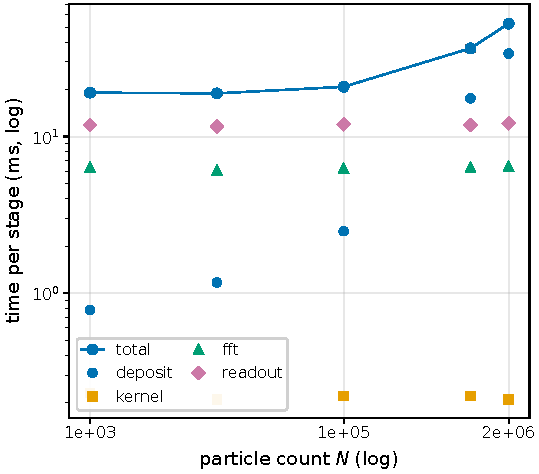
\includegraphics[width=0.62\linewidth]{figs/F_a_scaling_vs_N.pdf}\\[2pt]
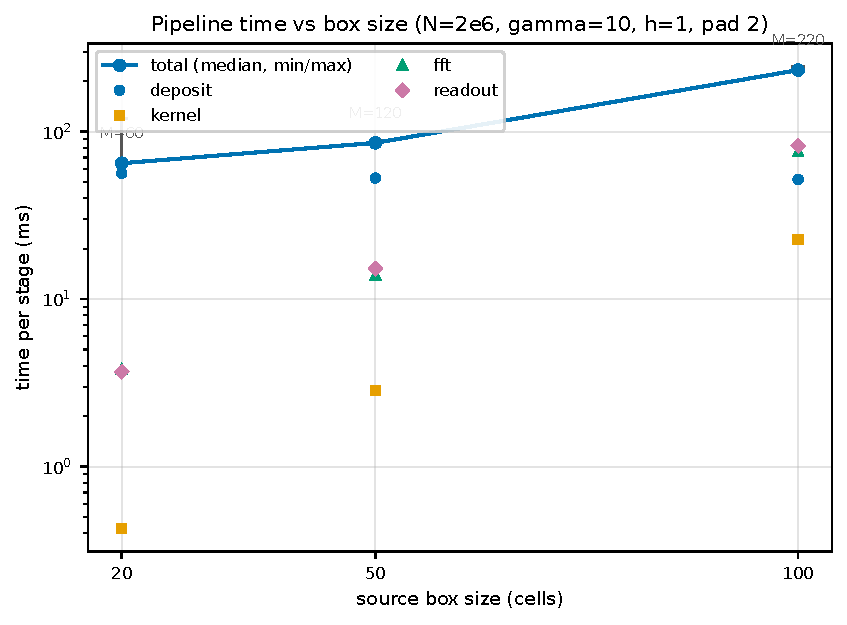
\includegraphics[width=0.62\linewidth]{figs/F_b_scaling_vs_box.pdf}
\caption{Pipeline time versus particle count (top, log-log) and source-box
size (bottom, semi-log), padded array $M=60/120/220$ cells, $\gamma=10$,
$h=1$, double precision, \texttt{rosi\_v100}/CUDA 12.6. Blue is the total
and markers the per-stage medians; the deposit dominates at
$N=2\times10^6$ ($57$ of $64.8$\,ms), and the total rises from $64.8$ to
$233$\,ms as $M$ grows from $60$ to $220$.}
\label{fig:Fa}
\end{figure}

Figure~\ref{fig:Fa} sweeps one axis at a time: the top panel fixes the
20-cell box and varies $N$, the bottom panel fixes $N=2\!\cdot\!10^6$ and
varies the box. The scaling is in two regimes, with the crossover set by
the box, not the particle count. At large $N$ the deposit dominates, linear
in $N$, $52$--$57$ ms on the $2\times10^6$ rows while the FFT, kernel, and
read-out stay under $10$ ms at the $20$-cell box; the total is flat across
$\gamma=1,10,100$ ($64.9/64.4/64.8$ ms). At large boxes the kernel and FFT
scale with $M^3$: from $M=60$ to $M=220$ the total goes from $64.8$ ms to
$233$ ms, and halving $h$ costs $1.07\times$ and $2.35\times$ because the
deposit stays constant. The per-$h$ totals are $64.76$, $69.27$, and
$151.51$ ms for $h=1$, $1/2$, $1/4$ (padded array $M=60/100/180$,
$2\times10^6$ particles, 20-cell box). On the H100 (\texttt{jrc0880},
\texttt{sm\_90}), the same $2\times10^{6}$, $20$-cell, $h=1$ mesh is
$0.052$\,s compute (deposit $34.4$\,ms, kernel $1.08$\,ms, FFT $7.44$\,ms,
read-out $9.02$\,ms; medians of three), and $0.755$\,s CLI wall including
the particle read and the HDF5 write.

\begin{table}[t]
\centering
\small
\caption{Per-stage medians (ms) and device allocation (MiB), padding 2,
double, \texttt{rosi\_v100} GPU 0. ``box'' is the source-box size in cells;
$M$ is the padded FFT array per axis. Stage columns are medians over the
three timed repeats.}
\label{tab:matrix}
\begin{tabular}{lrrrrrrrrrrr}
\toprule
$N$ & box & $\gamma$ & $h$ & $n$ & $M$ & total & deposit & kernel & FFT & read-out & dev \\
\midrule
$10^3$   & 20  & 10  & 1   & 30  & 60  & 10.17  & 1.13  & 0.48 & 4.36  & 4.08  & 8.4  \\
$10^4$   & 20  & 10  & 1   & 30  & 60  & 10.69  & 2.42  & 0.53 & 4.37  & 3.35  & 8.7  \\
$10^5$   & 20  & 10  & 1   & 30  & 60  & 12.90  & 4.59  & 0.48 & 4.07  & 3.28  & 11.4 \\
$10^6$   & 20  & 10  & 1   & 30  & 60  & 61.92  & 53.61 & 0.53 & 4.31  & 3.45  & 38.9 \\
$2\!\cdot\!10^6$ & 20  & 10  & 1   & 30  & 60  & 64.76  & 56.51 & 0.43 & 3.80  & 3.69  & 69.4 \\
$2\!\cdot\!10^6$ & 50  & 10  & 1   & 60  & 120 & 85.67  & 52.82 & 2.85 & 13.89 & 15.20 & 127.4 \\
$2\!\cdot\!10^6$ & 100 & 10  & 1   & 110 & 220 & 232.97 & 51.89 & 22.66 & 75.97 & 82.40 & 468.7 \\
$2\!\cdot\!10^6$ & 20  & 10  & 1/2 & 50  & 100 & 69.27  & 52.38 & 1.29 & 7.43  & 8.16  & 99.5  \\
$2\!\cdot\!10^6$ & 20  & 10  & 1/4 & 90  & 180 & 151.51 & 50.94 & 11.76 & 43.38 & 44.58 & 284.5 \\
\bottomrule
\end{tabular}
\end{table}

No configuration came near the $32$ GB device limit; the largest exact
device allocation was $468.7$ MiB. Memory scales with the padded bunch box,
not the global field.

\begin{table}[t]
\centering
\small
\caption{End-to-end pipeline time including the checkpoint writer and the
openPMD reader, medians over 3 repeats, \texttt{rosi\_v100} GPU 0, 20-cell
box, $\gamma=10$, CLI \texttt{--tolerance} $10^{-3}$. A different
measurement path from the compute-only Table~\ref{tab:matrix}: the totals
include the writer (the dominant added term); the per-stage split is
deposit/kernel/FFT/readout/writer.}
\label{tab:e2e}
\begin{tabular}{lrrrrrr}
\toprule
$N$ & total & deposit & kernel & FFT & readout & write \\
\midrule
$10^{4}$  & 22.00 & 2.70  & 0.53 & 4.53 & 3.06 & 11.29 \\
$10^{5}$  & 24.87 & 5.82  & 0.56 & 4.31 & 3.80 & 10.65 \\
$10^{6}$  & 47.15 & 31.56 & 0.46 & 4.20 & 3.95 & 7.54  \\
\bottomrule
\end{tabular}
\end{table}

Table~\ref{tab:e2e} is the same pipeline with the writer in the loop. The
deposit is still linear in $N$ ($2.70\to31.56$ ms from $10^4$ to $10^6$),
and the FFT is still box-bound and flat. The writer is the dominant added
term: $11.29$ ms at $10^4$ and $7.54$ ms at $10^6$. The $N=10^6$ total is
$47.15$ ms with the writer, versus $61.92$ ms in the compute-only
Table~\ref{tab:matrix}; the two campaigns differ in measurement path and
timing boundary, so neither is the other's total plus the writer.

\subsection{MPI rank scaling}
\label{sec:mpi-scale}

The rank-parallel compute and the collective writer were remeasured on
\texttt{jureca-h100} (four H100 PCIe 80\,GB, sm\_90, CUDA 13.4,
medians of three serialized runs).  The mesh stage
(deposit + kernel + FFT + read-out) at $N=2\times10^{6}$, $256^3$ takes
$581$, $411$ and $325$\,ms at $1$, $2$ and $4$ ranks ($1.41\times$ and
$1.79\times$); the replicated deposit and source spectrum cap the speedup.
The fast-GPU near shell at $32^3$, $R=1.5$, tile 8 takes $519$, $653$ and
$1112$\,ms: at this small size the tile split and the correction all-reduce
dominate, so more ranks do not help.  The collective HDF5 writer at
$256^3$ takes $3319$, $3327$ and $3323$\,ms at $1$, $2$ and $4$ ranks
($1.00\times$), essentially flat and the dominant part of the total.

\begin{table}[t]
\centering
\small
\caption{Rank scaling on \texttt{jureca-h100}, medians of three serialized
runs.  Mesh: $N=2\times10^{6}$, $256^3$, component-parallel (replicated
deposit and source FFT).  Near shell: $N=200$, $32^3$, $R=1.5$, tile 8,
tile-parallel, fast-GPU.  Write: $256^3$, collective HDF5.  The near-shell
column is a small-size case where the all-reduce dominates; the mesh and
writer are the production-relevant columns.}
\label{tab:mpi}
\begin{tabular}{lccc|cc|cc}
\toprule
 & \multicolumn{3}{c}{near shell} & \multicolumn{2}{c}{mesh} & \multicolumn{2}{c}{write} \\
\cmidrule(lr){2-4}\cmidrule(lr){5-6}\cmidrule(lr){7-8}
ranks & wall (ms) & speedup & eff.\ & wall (ms) & speedup & wall (ms) & speedup \\
\midrule
1 & $519.4$ & $1.00$ & $100\%$ & $581$ & $1.00$ & $3319$ & $1.00$ \\
2 & $652.9$ & $0.80$ & $40\%$  & $411$ & $1.41$ & $3327$ & $1.00$ \\
4 & $1112.2$ & $0.47$ & $12\%$ & $325$ & $1.79$ & $3323$ & $1.00$ \\
\bottomrule
\end{tabular}
\end{table}

\begin{figure}[H]
\centering
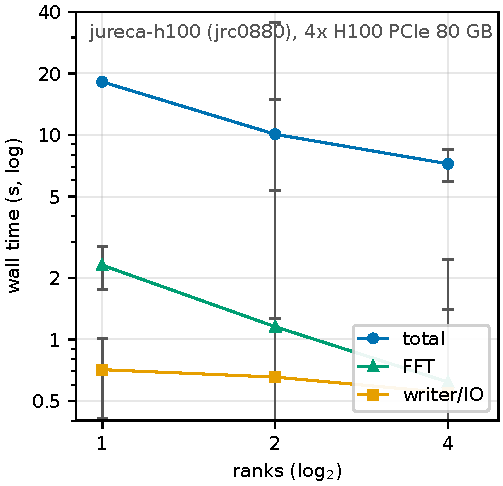
\includegraphics[width=0.58\linewidth]{figs/F_mpi_rank_scaling_h100.pdf}
\caption{Strong scaling of the three rank-parallel pieces on
\texttt{jureca-h100} for $1$--$4$ ranks, medians of three serialized runs:
near shell ($32^3$, $R=1.5$, tile 8), mesh ($2\times10^{6}$ particles,
$256^3$), and the collective writer ($256^3$).  The writer is flat; the
mesh reaches $1.79\times$; the small near-shell case has all-reduce
overhead and does not scale.}
\label{fig:h100mpiscaling}
\end{figure}

\paragraph{Distributed-mode scaling and its limits.}
The writer column above is the replicated path: only rank 0 writes the full
field, so it cannot scale by construction.  Forcing the slab-local production
mode (\texttt{--fft-mode distributed}) at $256^3$, $N=2\times10^{6}$, gives a
total of $21.6$, $12.3$ and $13.0$\,s and a writer of $4.19$, $2.88$ and
$6.46$\,s at $1$, $2$ and $4$ ranks; the FFT is $2.30$, $1.16$ and
$0.63$\,s.  The writer scales to two ranks ($1.45\times$) and regresses at
four ($0.65\times$), a collective-HDF5 contention on the shared series, not a
serialisation in picBunch.  The near shell partitions tiles but still
all-reduces the full correction array; at $32^3$ that communication and the
tile imbalance dominate, which is why the near-shell column reverses.  A
local-slab reduction and a writer with per-rank contiguous slabs are the
required fixes for many-rank runs.

\begin{table}[t]
\centering
\small
\caption{Distributed-mode strong scaling, $256^3$, $N=2\times10^{6}$,
medians of three serialized runs.  The writer is the collective HDF5 series;
the replicated writer (only rank 0 writes) is flat by construction and is not
shown here.}
\label{tab:h100dist}
\begin{tabular}{lrrr}
\toprule
 & 1 rank & 2 ranks & 4 ranks \\
\midrule
total (s)   & $21.6$ & $12.3$ & $13.0$ \\
FFT (s)     & $2.30$ & $1.16$ & $0.63$ \\
writer (s)  & $4.19$ & $2.88$ & $6.46$ \\
\bottomrule
\end{tabular}
\end{table}

\subsection{H100 remeasurement}
\label{sec:h100}

A fresh campaign on \texttt{jureca-h100} (four H100 PCIe 80\,GB, sm\_90,
CUDA 13.4, serialized on one GPU, medians of three runs) reproduces the
scaling picture with current hardware.  At $N=2\times10^{6}$, a 20-cell box
takes $60.5$\,ms end to end (deposit $36.1$, FFT $1.53$, read-out $17.5$,
writer $5.1$\,ms); a 100-cell box takes $147.9$\,ms (deposit $38.9$, FFT
$31.3$, read-out $21.4$, writer $53.8$\,ms).  The deposit remains linear in
$N$; the 100-cell case is FFT- and writer-bound.  For $N=200$ particles the
16- and 64-bin multi-velocity runs take $92.2$ and $100.6$\,ms; the $B_z$
peak differs by $4.6\%$, within the shot noise of 200 particles.

Rank scaling at $N=2\times10^{6}$ and the near-shell case are in
Section~\ref{sec:mpi-scale}: the shared HDF5 writer dominates the total and
is flat across ranks, while the mesh stage reaches $1.79\times$ at four
ranks.

\begin{table}[t]
\centering
\small
\caption{H100 remeasurement, medians of three serialized runs.  Top:
$N=2\times10^{6}$, one bin, one rank, stage times in ms.}
\label{tab:h100}
\begin{tabular}{lrrrrr}
\toprule
box & deposit & FFT & read-out & writer & total \\
\midrule
20 cells  & $36.1$ & $1.53$ & $17.5$ & $5.1$  & $60.5$ \\
100 cells & $38.9$ & $31.3$ & $21.4$ & $53.8$ & $147.9$ \\
\bottomrule
\end{tabular}

\end{table}

\section{Limitations}
\label{sec:limits}

The mesh is a far-field method. Its limits are set by $r/h$ and $\gamma$,
and they are measured, not assumed. The mesh alone does not reach $10^{-3}$
where the slices cut the bunch core (Section~\ref{sec:slices}); that is the
single-mesh limitation the slices display. The opt-in near shell
(Section~\ref{sec:nearsheet}) assembles exactly to roundoff, so at the
measured radii the residual is the mesh outside the shell, not the tile
subtraction. The perpendicular direction at $\gamma=10$ does not converge at
the natural cell size: $1.5\times10^{-2}$ at $d=48$, aspect 1, against the
point field, of which the TSC smoothing alone is $1.48\times10^{-2}$
(Table~\ref{tab:d48}) \citep{N2b,D11}. At $\gamma=100$ the perpendicular error
is $3.75\times10^{-1}$ at $d=48$ and does not converge as $d$ grows
\citep{N2b,D8}. At aspect 4, $\gamma=1$ already fails the gate at $d=48$
($2.4\times10^{-3}$) \citep{N2b}. The measured near-shell cost ladder does
not fit the $2\times10^{6}$ / $10^{-3}$ / $300$\,s envelope at production
size (Section~\ref{sec:cost}). The detailed discussion is in
Section~\ref{sec:discussion}.

\section{Accuracy}
\label{sec:accuracy}

Each error figure names its reference (M mesh, T continuum, P point). The three
references stay apart throughout:
the mesh $M$, the TSC-convolved continuum $T$ (Eq.~\eqref{eq:Fc}, the
quantity the mesh is built to compute), and the point field $P$ (the
un-smoothed Li\'enard--Wiechert field). $M$ against $T$ is the discrete
deposit and convolution error. $T$ against $P$ is the TSC smoothing, an
$O(1)$ effect at $\gamma h \gg 1$. $M$ against $P$ is the total.

\subsection{The reference and the two metrics}

The arbiter is an independent TSC-convolved continuum, a tensor
Gauss--Legendre quadrature with a TSC-knot split and a singularity-cancelling
power map \citep{indfield}. Its quadrature error is below the
$3\times10^{-4}$ gate in every configuration measured here \citep{N2b}.

Two metrics are reported and are not interchangeable. The judge metric
$|\mathrm{ref}-\mathrm{mesh}|/(1+\max(|\mathrm{ref}|,\mathrm{mesh}|))$ is
absolute-dominated: for fields of order $10^{-9}$ V/m the $+1$ denominator
swamps the error, so it reports a crossover at $d=2$ for every case and does
not discriminate \citep{W4b}. The relative per-component error
$|\mathrm{ref}-\mathrm{mesh}|/\max(|\mathrm{ref}|,\mathrm{mesh}|)$, over
components where $|\mathrm{ref}|\ge10^{-3}$ of the local field, is the
meaningful one. This section reports relative error as the metric of record.

\subsection{Reference-separated error at $d=48$}

\begin{table}[t]
\centering
\small
\caption{L2-pooled relative error at $d=48$ cells, $h=1$, perpendicular
direction (L2 over the six components; the single-component worst for
$\gamma=1$, aspect 4, $M\!-\!T$ is $2.65\times10^{-5}$ and for
$\gamma=10$, aspect 1 is $1.4\times10^{-3}$) \citep{N2b}.
$M\!-\!T$: mesh vs TSC-convolved continuum (the target). $M\!-\!P$: mesh vs
point field. $T\!-\!P$: TSC smoothing, mesh-independent. At $\gamma=10$,
aspect 1, the gap between $M\!-\!P$ and $M\!-\!T$ is the smoothing
($1.5\times10^{-2}$ vs $2.6\times10^{-4}$, an L2 ratio of $58\times$), not
the mesh.}
\label{tab:d48}
\begin{tabular}{lrrrr}
\toprule
$\gamma$ & aspect & $M\!-\!T$ & $M\!-\!P$ & $T\!-\!P$ \\
\midrule
1   & 1 & $1.38\times10^{-7}$ & $9.89\times10^{-8}$ & $3.96\times10^{-8}$ \\
1   & 4 & $2.65\times10^{-5}$  & $2.39\times10^{-3}$  & $2.40\times10^{-3}$  \\
10  & 1 & $2.6\times10^{-4}$    & $1.5\times10^{-2}$   & $1.48\times10^{-2}$  \\
10  & 4 & $3.33\times10^{-2}$  & $1.19\times10^{-1}$  & $1.44\times10^{-1}$  \\
100 & 1 & $3.75\times10^{-1}$  & $2.20\times10^{-1}$  & $4.40\times10^{-1}$  \\
100 & 4 & $2.78\times10^{0}$   & $2.49\times10^{-1}$  & $8.32\times10^{-1}$  \\
\bottomrule
\end{tabular}
\end{table}

Table~\ref{tab:d48} shows two things. At $\gamma=10$, aspect 1, the mesh
against the point field ($M\!-\!P=1.5\times10^{-2}$) is about $58\times$ the
mesh against its own target ($M\!-\!T=2.6\times10^{-4}$, an L2 ratio); the
difference is
the TSC smoothing, which $M\!-\!P$ inherits and $M\!-\!T$ does not. A
mesh-versus-point comparison measures the shape the deposit applies, not the
discretization error. Second, the $M\!-\!T$ error is not converged
perpendicular to the beam at $\gamma h \gg 1$: at aspect 1 it is acceptable
only for $\gamma=10$ and not for $\gamma=100$; at aspect 4 it is not
converged at any $\gamma$. Only the axial direction is clean at every
$\gamma$ \citep{N2b}.

\subsection{The independent validation}

A second, independent pass measured the shipped CLI end to end:
\texttt{picBunch} at \texttt{bfaa1e26} (field path unchanged through
v0.1.3), rosi\_v100, \texttt{indfield.py}
order $12$ refine $3$, $d=2$ to $32$ cells, $\gamma\in\{1,10\}$, aspect 1
and 4, single particle and three-particle cloud \citep{W4b}.

\begin{table}[t]
\centering
\small
\caption{Worst per-component relative error (over $x,y$, $|\mathrm{ref}|
\ge10^{-3}$ of the local field) of the shipped CLI against the
TSC-convolved continuum, at $d=16$ and $d=32$ cells; rosi\_v100,
\texttt{indfield.py} order $12$ refine $3$ \citep{W4b}. ``s/c'' = single /
cloud. $\gamma=10$ does not cross $3\times10^{-4}$ within $32$ cells;
$\gamma=1$ crosses at $d=12$ (aspect 1) and $d=32$ (aspect 4).}
\label{tab:w4b}
\begin{tabular}{llrr}
\toprule
$\gamma$, aspect & s/c & $d\!=\!16$ & $d\!=\!32$ \\
\midrule
1, 1  & $3.5\mathrm{e}{-5}$ / $1.0\mathrm{e}{-4}$ & $2.2\mathrm{e}{-6}$ / $2.0\mathrm{e}{-5}$ \\
1, 4  & $2.8\mathrm{e}{-3}$ / $2.1\mathrm{e}{-3}$ & $2.0\mathrm{e}{-4}$ / $2.6\mathrm{e}{-4}$ \\
10, 1 & $5.6\mathrm{e}{-2}$ / $5.3\mathrm{e}{-2}$ & $6.3\mathrm{e}{-3}$ / $6.5\mathrm{e}{-3}$ \\
10, 4 & $5.5\mathrm{e}{-2}$ / $5.0\mathrm{e}{-2}$ & $6.3\mathrm{e}{-3}$ / $6.4\mathrm{e}{-3}$ \\
\bottomrule
\end{tabular}
\end{table}

Table~\ref{tab:w4b} confirms the reference-separated picture independently.
$\gamma=1$ crosses $3\times10^{-4}$ at $d=12$ (aspect 1, $1.1\times10^{-4}$)
and $d=32$ (aspect 4, $2.6\times10^{-4}$); at $\gamma=10$ the relative error
floors near $6\times10^{-3}$ at $d=32$ for all four cases and does not cross
$3\times10^{-4}$ within the swept range. The near shell is far worse, with
relative error $O(0.4)$--$0.8$ at $d=2$. The window starts at $d=2$, so the
TSC support interior ($|s|<1.5$ cells) is not covered \citep{W4b}.

\begin{figure}[t]
\centering
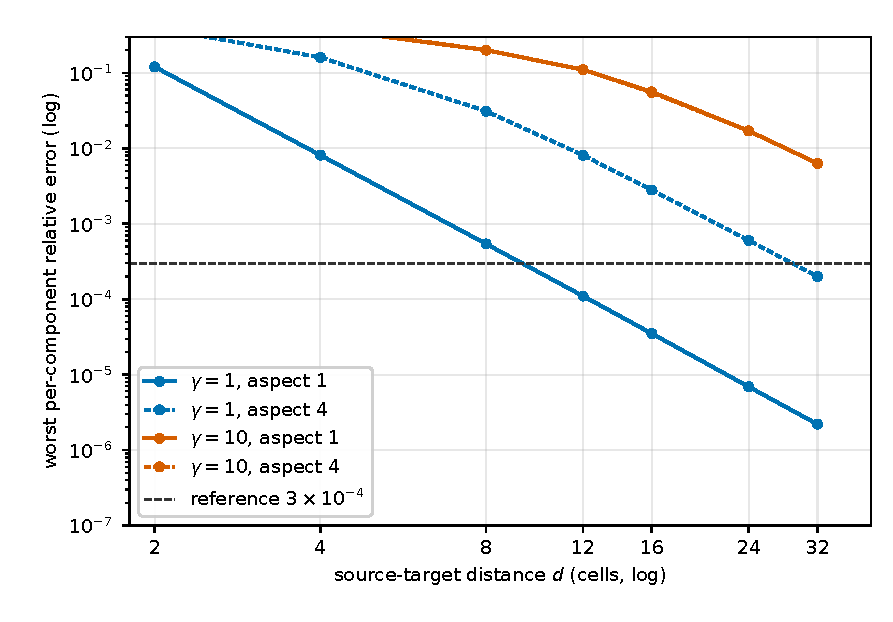
\includegraphics[width=0.95\linewidth]{figs/F_w4b_rel_error.pdf}
\caption{Worst per-component relative error of the shipped CLI against the
TSC-convolved continuum, per $d$ in cells, single-particle series only (the
three-particle cloud is in Table~\ref{tab:w4b}); rosi\_v100,
\texttt{indfield.py}
order $12$ refine $3$ \citep{W4b}. Solid, $\gamma=1$; dashed, $\gamma=10$;
blue, aspect 1; orange, aspect 4. $\gamma=1$ crosses the $3\!\cdot\!10^{-4}$
gate at $d=12$ (aspect 1) and $d=32$ (aspect 4); $\gamma=10$ floors near
$6\!\cdot\!10^{-3}$ at $d=32$ and never crosses within the swept range.}
\label{fig:Fw4b}
\end{figure}

The point-field column (Table~\ref{tab:d48}, $M\!-\!P$) is the mesh against
the un-smoothed field. It carries the TSC smoothing in addition to the deposit
error, and the two never agree for $\gamma h \gg 1$. The first half's distance
sweep (Fig.~\ref{fig:Fw4b}) plots this point-field comparison; the
$M\!-\!T$ column of Table~\ref{tab:d48} is the mesh against its own target.

\subsection{Crossover radii}

\begin{table}[t]
\centering
\small
\caption{Crossover radius in cells: first $d$ at which every larger $d$ is at
or below the gate, $h=1$, L2 over the six components, per axis direction,
worst over the three positive axis directions ($>$48: not reached)
\citep{N2b}. $T$: TSC-convolved continuum; $P$: point field. Oblique
directions are $\sim1.5\times$ larger. The $\gamma=1$ aspect 1 row is $d=8$
against both references here, versus the $d=12$ of the shipped-CLI series in
Table~\ref{tab:w4b}: the two measurements use different component sets (six
axis directions, L2-pooled, versus the per-component relative error over
$x,y$) and different implementations (the N2b standalone measurement versus
the shipped executable), so they are not the same crossover
\citep{N2b,W4b}.}
\label{tab:crossover}
\begin{tabular}{lcc|cc|cc}
\toprule
 & \multicolumn{2}{c}{$3\!\times\!10^{-4}$} & \multicolumn{2}{c}{$10^{-3}$} \\
\cmidrule(lr){2-3}\cmidrule(lr){4-5}
$\gamma$ & aspect & ref & axial $z$ & perp $x$ & axial $z$ & perp $x$ \\
\midrule
1   & 1 & $T$ & 8  & 8  & 6  & 6  \\
    & 1 & $P$ & 8  & 8  & 6  & 6  \\
1   & 4 & $T$ & 6  & 24 & 6  & 16 \\
    & 4 & $P$ & 48 & $>48$ & 32 & $>48$ \\
10  & 1 & $T$ & 6  & 48 & 6  & 48 \\
    & 1 & $P$ & $>48$ & $>48$ & 32 & $>48$ \\
10  & 4 & $T$ & 6  & $>48$ & 6  & $>48$ \\
    & 4 & $P$ & $>48$ & $>48$ & 32 & $>48$ \\
100 & 1 & $T$ & 6  & $>48$ & 6  & $>48$ \\
    & 1 & $P$ & $>48$ & $>48$ & 32 & $>48$ \\
100 & 4 & $T$ & 6  & $>48$ & 6  & $>48$ \\
    & 4 & $P$ & $>48$ & $>48$ & 32 & $>48$ \\
\bottomrule
\end{tabular}
\end{table}

At $\gamma=1$, aspect 1, the mesh is within $3\times10^{-4}$ of both
references from $d=8$; the two are interchangeable there. From $\gamma=10$
up, against the point field the perpendicular direction does not reach
$3\times10^{-4}$ within $48$ cells; against the target the perpendicular
crossover is $48$ ($\gamma=10$, aspect 1) or not reached. The axial
direction stays at $6$ against the target at every $\gamma$ \citep{N2b}.

\subsection{The disagreement is per-source}

On a $64\times64\times32$, cell $10^{-7}$\,m, stationary bunch ($\gamma=1$),
the disagreement with the exact-quadrature reference does not grow with
particle count: outside the TSC support the worst per-component error stays
in the $10^{-3}$ to $3\times10^{-2}$ band across $N=1$ to $1000$
\citep{W7t}. The $O(1)$ values at $N\ge10$ occur only because the global
worst sample point falls $0.42$--$0.65$ cells from a source, inside that
source's TSC support. A flat per-source floor is what a kernel or
reference-type difference produces; a charge-weighting defect would grow with
$N$. The measured disagreement is the in-support, near-source regime, and it
does not depend on the number of sources \citep{W7t}.

\subsection{The $h^{3}$ defect and its correction}

Section~\ref{sec:method} derives the $h^{3}$ factor and the $1/h^{3}$
overshoot of the delivered mesh. Fig.~\ref{fig:Ff} is the measured
per-$h$ series, worst per-component relative error against
\texttt{indfield.py}, at fixed physical separation,
$\gamma\in\{1,10\}$, aspect 1 and 4, rosi\_v100. The per-$h$ runs are at
fixed physical separation, so they are not a scale-invariance demonstration
(Section~\ref{sec:scaleinvariance}); they show that the after-fix field is
stable to about $9\times10^{-4}$ over $h=1$ to $1/2$ (the refine gate,
below), while the pre-fix field, $1/h^{3}$ too large in absolute terms, has
a relative error that rises toward $1$ as $h$ is refined (only the absolute
error scales as $h^{-3}$; the relative error saturates because the
reference is not scaled with it) \citep{F4}.

\begin{figure}[t]
\centering
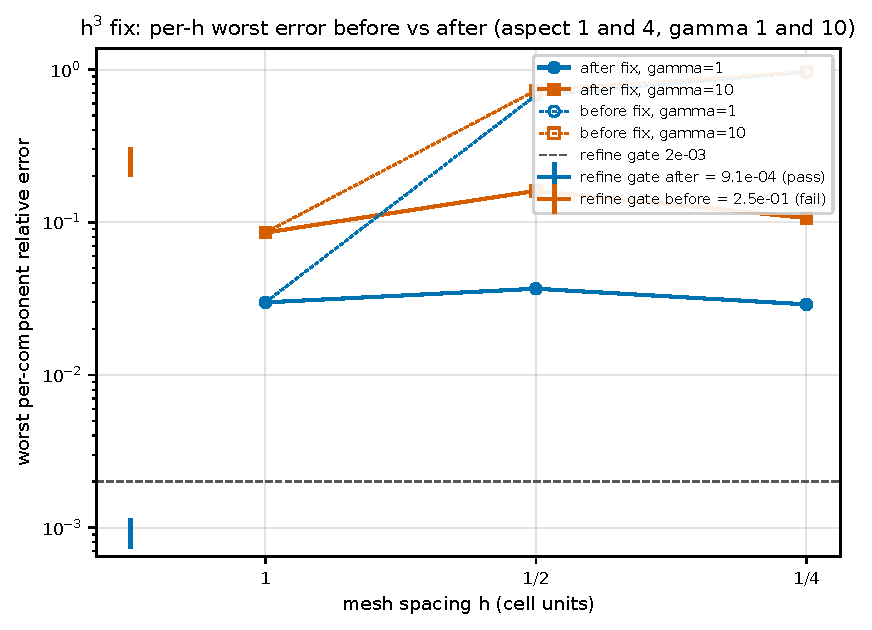
\includegraphics[width=0.95\linewidth]{figs/F_f_h3_regression.pdf}
\caption{Measured per-$h$ worst per-component relative error before and
after the $h^{3}$ fix (commit \texttt{fef43bbd}, branch
\texttt{experimental/mesh-h3}), at fixed physical separation,
$\gamma\in\{1,10\}$, aspect 1 and 4, rosi\_v100 \citep{F4}. Solid markers,
after the fix (stable to about $9\times10^{-4}$ over $h=1$ to $1/2$); open
markers, before the fix (relative error rises toward $1$ as $h$ is refined).
The vertical bars are the refine-gate values
$|\mathbf{h}\!=\!1-\mathbf{h}\!=\!1/2|/(1+\max)$:
$9.13\!\cdot\!10^{-4}$ after (gate $2\!\cdot\!10^{-3}$, pass) and
$2.48\!\cdot\!10^{-1}$ before (fail). At $h=1$ the pre- and post-fix fields
are byte-identical (sha256 \texttt{b6600}ec0\ldots) \citep{F4}.}
\label{fig:Ff}
\end{figure}

The correction is verified three ways \citep{F4}. The refinement gate
$|\mathbf{h}\!=\!1-\mathbf{h}\!=\!1/2|/(1+\max)$ is $9.13\times10^{-4}$
after the fix (pass) and $2.48\times10^{-1}$ before (fail). Against the
independent reference, the pre-fix absolute field is $1/h^{3}$ too large and
the pre-fix worst per-component relative error rises toward $1$ as $h$ is
refined: at $\gamma=1$, aspect 1 it is $6.90\times10^{-3}$ at $h=1$,
$6.78\times10^{-1}$ at $h=1/2$, and $9.63\times10^{-1}$ at $h=1/4$, while
the after-fix values are stable to about $9\times10^{-4}$ over $h=1$ to
$1/2$. (The aspect 4 series is $2.98\times10^{-2}$ at $h=1$,
$5.98\times10^{-1}$ at $h=1/2$, $9.41\times10^{-1}$ at $h=1/4$.) At $h=1$
the pre- and post-fix validate files are byte-identical, so the fix changes
nothing where the original was already correct.

\subsection{Determinism and the \texttt{gridUnitSI} defect}

Repeated runs of the shipped CLI are bit-identical: two runs of the same
input produce byte-identical E/B mesh payloads (md5 \texttt{d3641d64\ldots},
$15\,092\,736$ bytes) \citep{W4b}. The CLI also rejects a below-floor
\texttt{--tolerance} ($10^{-15}$) and a two-velocity input, each with exit 1
\citep{W4b}.

A defect found during this validation and fixed after v0.1:
\texttt{gridUnitSI} was applied twice. The reader converts the raw
\texttt{gridSpacing} to SI (\texttt{OpenPMD.cpp:505}), and the CLI
(\texttt{main.cpp:248}) multiplies by \texttt{gridUnitSI} a second time, so
the cell size is off by one factor of \texttt{gridUnitSI}. A mesh with
\texttt{gridUnitSI} $=10^{-6}$ and a physical cell of $10^{-6}$\,m yields a
cell of $10^{-12}$\,m and then aborts with
\texttt{cannot create std::vector larger than max\_size()}. Fixed in v0.1.1
with an end-to-end test that fails on the old code \citep{W4b}. This is a
lesson about reader-only unit tests: the reader-level conversion is correct,
but the composition at the CLI boundary is what the user sees, and it was
wrong.

\section{Cross-validation and checkpoint transport}
\label{sec:comparison}

Two independent checks constrain the method externally: a cross-validation
against PIConGPU's exact-quadrature field reference, and a checkpoint and
restart transport. Neither is a truth comparison.

\subsection{Cross-validation against the PIConGPU reference}

The reference is the TSC-convolved field (Section~\ref{sec:accuracy}),
evaluated in PIConGPU in its reference-only field-initializer mode
\citep{W7t}. picBunch is at
\texttt{339ca7ad} (\texttt{experimental/mvp}); \texttt{ctest} passes 10/10
\citep{W7r}. Both sides use identical Yee offsets, grid, and origin; the
reference staggered point maps to a picBunch node by index with zero snap
deviation \citep{W7r}.

At $318$ staggered points on a $64\times64\times32$ grid, cell
$10^{-7}$\,m, the overall worst per-component relative error is
$4.86\times10^{-2}$ for $\gamma=1$ ($E/z$) and $6.20\times10^{-1}$ for
$\gamma=10$ ($E/z$; $E/y$ is $5.16\times10^{-1}$), against a reference
reproducibility floor of $1.19\times10^{-6}$ ($E$) and
$1.43\times10^{-6}$ ($B$) \citep{W7r,D13}. picBunch is about four to six
orders of magnitude above that floor, a no-agreement statement at the
reference floor, not a defect: B is exactly zero for $\gamma=1$ in both, the
bulk agrees to below $1$--$3\%$, and the error is concentrated at the core
and the beamed peaks \citep{W7r,D13}.

The whole-field comparison, $N=1000$ on $32\times32\times16$, cell
$2\times10^{-7}$\,m, $16384$ nodes per component, gives the same picture:
$\gamma=1$ bulk median $3.8$--$7.8\times10^{-3}$ with an L2 of
$4.6$--$5.7\times10^{-2}$; $\gamma=10$ bulk median $1.4$--$3.3\times10^{-2}$
but a beamed-core overshoot that pushes the $E/y$, $E/z$ L2 to
$0.76$--$0.92$ \citep{W7r}. The forward $E/x$ is well resolved at
$\gamma=10$ ($\sim6\%$); the beamed transverse $E/y$, $E/z$ are
$50$--$130\%$ worst at the core, where the Lorentz-contracted field is a
sub-cell pancake that TSC and the spectral near-field kernel cannot resolve
\citep{W7r}.

\begin{table}[t]
\centering
\small
\caption{Whole-field comparison of picBunch against the PIConGPU
\texttt{referenceOnly} field, $N=1000$, $32\times32\times16$, cell
$2\times10^{-7}$\,m,
$16384$ nodes/component, rosi\_v100 \citep{W7r}. \texttt{worst\_rel} is
peak-normalized; median and p99 are per-point over nodes with
$|\mathrm{ref}|>10^{-3}\times$peak; L2 is pooled. Not a truth comparison.}
\label{tab:wholefield}
\begin{tabular}{lrrrr}
\toprule
component & worst\_rel & median & p99 & L2 \\
\midrule
\multicolumn{5}{l}{\emph{$\gamma=1$} (B identically 0)} \\
$E/x$ & $1.48\times10^{-1}$ & $3.92\times10^{-3}$ & $3.20\times10^{-1}$ & $4.62\times10^{-2}$ \\
$E/y$ & $1.49\times10^{-1}$ & $3.76\times10^{-3}$ & $2.93\times10^{-1}$ & $4.75\times10^{-2}$ \\
$E/z$ & $1.22\times10^{-1}$ & $7.81\times10^{-3}$ & $3.65\times10^{-1}$ & $5.67\times10^{-2}$ \\
\midrule
\multicolumn{5}{l}{\emph{$\gamma=10$} (B/x identically 0)} \\
$E/x$ & $1.36\times10^{-1}$ & $4.80\times10^{-3}$ & $1.23\times10^{-1}$ & $4.44\times10^{-2}$ \\
$E/y$ & $1.98$  & $1.36\times10^{-2}$ & $7.25$ & $7.63\times10^{-1}$ \\
$E/z$ & $1.93$  & $3.33\times10^{-2}$ & $10.1$ & $9.19\times10^{-1}$ \\
$B/y$ & $4.42\times10^{-1}$ & $3.12\times10^{-2}$ & $1.41$ & $2.58\times10^{-1}$ \\
$B/z$ & $4.63\times10^{-1}$ & $1.52\times10^{-2}$ & $0.93$ & $2.20\times10^{-1}$ \\
\bottomrule
\end{tabular}
\end{table}

\paragraph{Caveat: the sampling groups are distance-from-centroid.} The
$318$-point groups (inside-support, face, outside) were cut by distance from
the bunch centroid, in a bunch with a $\sim6$-cell spread \citep{D13}. That
grouping may understate how close the ``outside'' points actually are to a
source's TSC support, so the per-group numbers are a spatial profile, not a
clean inside/outside-of-support split. The per-source dependence in
Section~\ref{sec:accuracy} uses the explicit support union and is the
measurement that separates the per-source floor from any superposition
contribution \citep{W7t}.

\subsection{Checkpoint format and bitwise arrival}

The checkpoint writer emits a PIConGPU openPMD field checkpoint matching
PIConGPU's own plugin schema: root layout, openPMD version 5.0, $E$, $B$
$x/y/z$ at the exact Yee positions, grid spacing and offset, and the
\texttt{picongpu\_idProvider} mesh metadata \citep{W7B}. The default
precision is uniform \texttt{float32} for every field and particle record, so
a stock single-precision PIConGPU can load the file \citep{IMPL3}.
\texttt{v0.5.0} copies every species from the input bunch and carries a single
checkpoint-wide \texttt{picongpu\_idProvider} range \citep{INT1,FIX1,INT2};
the \texttt{charge} and \texttt{mass} records are written rather than omitted,
and the species is a single particle patch (Section~\ref{sec:interface}). The
remaining differences against a genuine PIConGPU checkpoint are non-blocking
metadata \citep{W7B}.

Field arrival is bitwise. A fresh \texttt{v0.5.0} checkpoint written from a
two-species input (16 electrons and 16 ions, \texttt{picongpu\_idProvider}
startId $0$, nextId $32$) restarts in PIConGPU with exit $0$ under both
\texttt{patch} modes (\texttt{bbox}: offset $(7,8,3)$, extent $(8,10,6)$;
\texttt{domain}: offset $(0,0,0)$, extent $(24,24,12)$), all six field
components bitwise-equal, $\max_\mathrm{abs\ diff} = 0.0$, electrons with ids
$0$ to $15$, first-step displacement exactly $\beta c\,dt$ with
$\beta = 0.9949874367$ \citep{INT2}. A validation-only build with the field
solver set to \texttt{None} loads the checkpoint and writes step 1; all six
components are bitwise-equal, max ULP $0$ \citep{W7B}.

\subsection{PML passthrough and the restart fixes}

On a $24\times24\times12$ deck the restart is exit $0$ with
\texttt{--periodic 1 1 1}, and the $16$ electrons load; initialization drops
from the $\sim116$\,s neuralBunch path to $1.8$\,s because the checkpoint
carries the field \citep{W7B}. The same investigation found the defects in
PIConGPU's restart path that the fixes PR addresses \citep{D15}:
\texttt{RestartFieldLoader} never reads \texttt{unitSI},
\texttt{gridSpacing} or \texttt{gridGlobalOffset}; the PML slabs are
unconditional; a successful restart suppresses the initial dump; and the
openPMD backend does not convert dataset dtypes. The fixes PR
(\texttt{psychocoderHPC-bot/picongpu} PR \#25, draft) adds restart metadata
validation, unitSI conversion, optional PML slabs, and an explicit dtype
contract, verified by real restarts including a factor-2 unitSI case
\citep{D15}.

\section{Discussion and limitations}
\label{sec:discussion}

The method computes the present-time field of a uniformly moving, TSC-shaped
bunch as a free-space FFT convolution. It is a far-field method.

\paragraph{What it is good for.} In the far field the relative error against
the point field is below $10^{-3}$ on the beam axis from $d=6$ for every
$\gamma$ \citep{N2b}. Against the TSC-convolved continuum: $\gamma=1$, aspect
1 crosses $3\times10^{-4}$ at $d=12$ ($1.1\times10^{-4}$); $\gamma=1$, aspect
4 at $d=32$ ($2.6\times10^{-4}$); $\gamma=10$ is $6.5\times10^{-3}$ at $d=32$,
not below $3\times10^{-4}$ within $48$ cells \citep{W4b,V2b}. At
$2\times10^{6}$ particles in a $20$-cell box the compute-only total is
$64.8$\,ms, dominated by the deposit ($56.5$\,ms), and flat in $\gamma$
\citep{SB1}. Repeated runs are bit-identical (md5 \texttt{d3641d64\ldots});
the Coulomb limit reproduces the TSC-convolved Coulomb field to
$4.88\times10^{-14}$ \citep{W4b,coulomb}.

\paragraph{What it is not.} The mesh alone does not reach $10^{-3}$ where the
slices cut the bunch core: on the $N=1000$ slice geometry the mesh-only worst
per-component plane error is $0.12$--$0.41$ for $\gamma=1$ and
$0.11$--$4.60$ for $\gamma=10$ (Table~\ref{tab:slices}). The exact near shell
(Section~\ref{sec:nearsheet}) is opt-in and its assembly is exact to roundoff;
at the measured $R=3/4$ radii on the $h=1$ slice grid the residual is the mesh
outside the shell, not the tile subtraction
(Section~\ref{sec:slices-runs}). The perpendicular direction at $\gamma=10$
does not converge at the natural cell size ($1.5\times10^{-2}$ at $d=48$,
aspect 1; the TSC smoothing alone is $1.48\times10^{-2}$,
Table~\ref{tab:d48}), and reaching $10^{-3}$ perpendicular at $r=8$ cells would
need $h\approx1/29$, a $2.4\times10^{4}$-fold increase in $M^{3}$ FFT work
\citep{N2b,D11}. At aspect 4, $\gamma=1$ already fails the gate at $d=48$
($2.4\times10^{-3}$) \citep{N2b}. The cross-validation confirms the same
boundary: the mesh does not agree with the exact reference at the reference
floor; the disagreement is per-source, in the TSC support, and does not grow
with particle count \citep{W7t,D13}.

\paragraph{Performance.} The cost is two regimes with a crossover set by the
box, not the particle count \citep{SB1}. At large $N$ the deposit dominates,
linear in $N$, $52$--$57$\,ms on the $2\times10^{6}$ rows. At large boxes the
FFT and kernel dominate: from $M=60$ to $M=220$ the total goes from
$64.8$\,ms to $233$\,ms, and halving $h$ costs $1.07\times$ and $2.35\times$
\citep{SB1}. The compute timings are single-GPU on one \texttt{rosi\_v100}
host. The output path has a multi-rank measurement: at $512^{3}$, tolerance
$10^{-3}$, the chunked writer runs in $54.3$\,s for one rank and $43.2$\,s
for two, the six datasets bitwise identical
(Section~\ref{sec:mpi-scale}) \citep{FIX1}. The near-field cost is a separate
wall: per-pair, $5.4\times10^{-5}$\,s for the ported stationary box8/rem8
evaluator, $3.1\times10^{-4}$\,s out of support and
$6.9\times10^{-3}$\,s in support for the accurate moving evaluator,
$1.62$\,s for the upstream adaptive settings
(Section~\ref{sec:cost}) \citep{K3}.

\paragraph{Scope.} The defensible scope, in floored relative per-component
error against the continuum, is $\gamma=1$ aspect 1 from $d=12$, $\gamma=1$
aspect 4 from $d=32$, and the axial component at $\gamma\le10$
\citep{W4b,N2b,D11}. The blanket statement ``$\gamma\le10$ meets $10^{-3}$''
is not supported: it fails perpendicular at the natural cell size,
$6.5\times10^{-3}$ at $\gamma=10$, $d=32$, aspect 1, still $1.8\times10^{-3}$
at $d=48$, not below $3\times10^{-4}$ within $48$ cells
\citep{W4b,N2b,V2b}. Each statement in Section~\ref{sec:accuracy} names which
metric (floored, unfloored, absolute) supports it; the floored column is
electric-only at $\gamma=10$ because the floor excludes the magnetic field,
and the judge metric $|\mathrm{ref}-\mathrm{mesh}|/(1+\max)$ reports $d=2$
for every case and does not discriminate. The radii in
Table~\ref{tab:crossover} are axis directions only; oblique directions are
$\sim1.5\times$ larger. Scale invariance
(Section~\ref{sec:scaleinvariance}) means only $r/h$ moves the error, so
reaching $10^{-3}$ at $r=8$ needs $h\approx1/29$
($2.4\times10^{4}$ times the $M^{3}$ nodes) \citep{N2b,D10}.

\section{Conclusion}
\label{sec:conclusion}

picBunch computes the present-time field of a uniformly moving, TSC-shaped
bunch as a zero-padded free-space FFT convolution with staggered Yee read-out,
and the discrete recipe, its measured cost, and its accuracy are given in full.
In relative per-component error against its TSC-convolved target, the mesh is
below $3\times10^{-4}$ from $d=12$ cells for $\gamma=1$, aspect 1, and from
$d=32$ for $\gamma=1$, aspect 4; at $\gamma=10$ it floors near
$6\times10^{-3}$ at $d=32$ and does not cross within the swept range
\citep{W4b}. The disagreement with the exact quadrature reference is per-source,
local to the TSC support, and independent of particle count. On periodic
decks the field round-trips bitwise through a real PIConGPU checkpoint and
restart: a solver=None validation load writes step 1 and all six components
are bitwise-equal, max ULP 0. The
method is a far-field tool: cheap, deterministic (md5 \texttt{d3641d64\ldots},
bit-identical repeats), and GPU-portable, with the near shell absent in v0.1
and the perpendicular direction at $\gamma\ge10$ not converged at the natural
cell size.


{\footnotesize\bibliography{refs}}

\end{document}
